%%%%%%%%%%%%%%%%%%%%%%%%%%%%%%%%%%%%%%%%%
% Arsclassica Article
% LaTeX Template
% Version 1.1 (10/6/14)
%
% This template has been downloaded from:
% http://www.LaTeXTemplates.com
%
% Original author:
% Lorenzo Pantieri (http://www.lorenzopantieri.net) with extensive modifications by:
% Vel (vel@latextemplates.com)
%
% License:
% CC BY-NC-SA 3.0 (http://creativecommons.org/licenses/by-nc-sa/3.0/)
%
%%%%%%%%%%%%%%%%%%%%%%%%%%%%%%%%%%%%%%%%%

%----------------------------------------------------------------------------------------
%	PACKAGES AND OTHER DOCUMENT CONFIGURATIONS
%----------------------------------------------------------------------------------------

\documentclass[
	11pt, % Main document font size
	a4paper, % Paper type, use 'letterpaper' for US Letter paper
	oneside, % One page layout (no page indentation)
	%twoside, % Two page layout (page indentation for binding and different headers)
	headinclude,footinclude, % Extra spacing for the header and footer
	BCOR5mm, % Binding correction
]{scrartcl}

%%%%%%%%%%%%%%%%%%%%%%%%%%%%%%%%%%%%%%%%%
% Arsclassica Article
% Structure Specification File
%
% This file has been downloaded from:
% http://www.LaTeXTemplates.com
%
% Original author:
% Lorenzo Pantieri (http://www.lorenzopantieri.net) with extensive modifications by:
% Vel (vel@latextemplates.com)
%
% License:
% CC BY-NC-SA 3.0 (http://creativecommons.org/licenses/by-nc-sa/3.0/)
%
%%%%%%%%%%%%%%%%%%%%%%%%%%%%%%%%%%%%%%%%%

%----------------------------------------------------------------------------------------
%	REQUIRED PACKAGES
%----------------------------------------------------------------------------------------

\usepackage[
nochapters, % Turn off chapters since this is an article        
beramono, % Use the Bera Mono font for monospaced text (\texttt)
eulermath,% Use the Euler font for mathematics
pdfspacing, % Makes use of pdftex’ letter spacing capabilities via the microtype package
dottedtoc % Dotted lines leading to the page numbers in the table of contents
]{classicthesis} % The layout is based on the Classic Thesis style

\usepackage{arsclassica} % Modifies the Classic Thesis package

\usepackage[T1]{fontenc} % Use 8-bit encoding that has 256 glyphs

\usepackage[utf8]{inputenc} % Required for including letters with accents

\usepackage{graphicx} % Required for including images
\graphicspath{{Figures/}} % Set the default folder for images

\usepackage{enumitem} % Required for manipulating the whitespace between and within lists

\usepackage{lipsum} % Used for inserting dummy 'Lorem ipsum' text into the template

\usepackage{subfig} % Required for creating figures with multiple parts (subfigures)

\usepackage{amsmath,amssymb,amsthm} % For including math equations, theorems, symbols, etc

\usepackage{varioref} % More descriptive referencing

%----------------------------------------------------------------------------------------
%	THEOREM STYLES
%---------------------------------------------------------------------------------------

\theoremstyle{definition} % Define theorem styles here based on the definition style (used for definitions and examples)
\newtheorem{definition}{Definition}

\theoremstyle{plain} % Define theorem styles here based on the plain style (used for theorems, lemmas, propositions)
\newtheorem{theorem}{Theorem}

\theoremstyle{remark} % Define theorem styles here based on the remark style (used for remarks and notes)

%----------------------------------------------------------------------------------------
%	HYPERLINKS
%---------------------------------------------------------------------------------------

\hypersetup{
%draft, % Uncomment to remove all links (useful for printing in black and white)
colorlinks=true, breaklinks=true, bookmarks=true,bookmarksnumbered,
urlcolor=webbrown, linkcolor=RoyalBlue, citecolor=webgreen, % Link colors
pdftitle={}, % PDF title
pdfauthor={\textcopyright}, % PDF Author
pdfsubject={}, % PDF Subject
pdfkeywords={}, % PDF Keywords
pdfcreator={pdfLaTeX}, % PDF Creator
pdfproducer={LaTeX with hyperref and ClassicThesis} % PDF producer
} % Include the structure.tex file which specified the document structure and layout
\usepackage[cm]{fullpage}
\usepackage[
	bottom=0.5in,
	top=   0.5in,
	left=  0.5in,
	right= 0.5in
]{geometry}
%\renewcommand*\rmdefault{cmr}

\hyphenation{Fortran hy-phen-ation} % Specify custom hyphenation points in words with dashes where you would like hyphenation to occur, or alternatively, don't put any dashes in a word to stop hyphenation altogether

\newtheorem*{hopkins}{Hopkins statistic} % Theorems

%----------------------------------------------------------------------------------------
%	TITLE AND AUTHOR(S)
%----------------------------------------------------------------------------------------

\title{\normalfont\spacedallcaps{clustering di wikipedia e relazione con le categorie degli articoli}} % The article title

\author{\spacedlowsmallcaps{Cazzaro Dalla Cia Lovisotto Vianello}}

\date{} % An optional date to appear under the author(s)

%----------------------------------------------------------------------------------------

\begin{document}

%----------------------------------------------------------------------------------------
%	HEADERS
%----------------------------------------------------------------------------------------

\renewcommand{\sectionmark}[1]{\markright{\spacedlowsmallcaps{#1}}} % The header for all pages (oneside) or for even pages (twoside)
%\renewcommand{\subsectionmark}[1]{\markright{\thesubsection~#1}} % Uncomment when using the twoside option - this modifies the header on odd pages
\lehead{\mbox{\llap{\small\thepage\kern1em\color{halfgray} \vline}\color{halfgray}\hspace{0.5em}\rightmark\hfil}} % The header style

\pagestyle{scrheadings} % Enable the headers specified in this block

%----------------------------------------------------------------------------------------
%	TABLE OF CONTENTS & LISTS OF FIGURES AND TABLES
%----------------------------------------------------------------------------------------

\maketitle % Print the title/author/date block

%\newpage

%----------------------------------------------------------------------------------------
%	INTRODUCTION
%----------------------------------------------------------------------------------------

\section{Introduzione}

Per il progetto del corso di Data Mining abbiamo deciso di svolgere la traccia proposta B, che proponeva di indagare fino a che punto un clustering sulle pagine di Wikipedia è consistente con le categorie associate alle pagine stesse.
Per fare ciò avevamo a disposizione due dataset, di differenti grandezze, formati da articoli di Wikipedia in lingua inglese.

A partire da tali premesse ci siamo prefissati i seguenti quesiti:

\begin{itemize}
	\item quanto sono clusterizzabili gli articoli del dataset?
	\item le categorie associate a questi articoli sono sensate?
	\item quali sono dei metodi validi per rappresentare opportunamente i nostri dati in input?
	\item come variano i cluster utilizzando tecniche diverse?
	\item c'è un numero ottimale di cluster per il dataset? Quanto vale?
	\item qual è il rapporto tra il cluster ottenuto e le categorie?
\end{itemize}

Tali quesiti troveranno risposta nel seguito della trattazione, che è strutturata nel modo che segue.
La sezione 2 illustra l'analisi preliminare effettuata sugli articoli e sulle categorie.
Successivamente il capitolo 3 descrive le tecniche utilizzate per rappresentare il dataset.
Il capitolo 4 tratta poi degli algoritmi di clustering applicati al dataset e delle tecniche di valutazione impiegate.
Di seguito la sezione 5 riporta e discute i risultati ottenuti nel capitolo precedente, offrendo anche un confronto tra i metodi utilizzati.
Infine la sezione 6 riassume il lavoro svolto, ciò che abbiamo ottenuto e propone alcuni spunti di ricerca per futuri sviluppi.


\section{Dataset e Analisi Preliminare}
	Ci sono stati messi a disposizione due dataset, di differenti grandezze, per effettuare questa analisi.
	Nello specifico abbiamo utilizzato quello minore, il quale è un \emph{dump} composto da un JSON contenente centomila articoli di Wikipedia in versione inglese.
	Per ogni articolo abbiamo a disposizione il titolo, il testo, l'id e le categorie dell'articolo.
	In particolare le categorie sono assegnate a discrezione degli autori e dei successivi revisori di ogni voce, in quanto Wikipedia non prevede una struttura o dei vincoli particolari per l'assegnazione di queste categorie.

	La nostra analisi mira a valutare la relazione semantica tra gli articoli e le loro categorie, quindi prima di effettuare l'analisi si è deciso di eliminare tutti gli articoli che non risultano essere associati a nessuna categoria. Queste pagine sono dette \emph{di disambiguazione} e quindi non sono utili per i nostri scopi.

	Per quanto concerne le categorie, una prima ispezione manuale rivela che esse sono alquanto arbitrarie e spesso così specifiche da essere associate ad un articolo soltanto.
	Esempio di ciò sono le categorie "Roads on the National Register of Historic Places in Illinois", "United Nations Security Council resolutions concerning Sudan" e "Singaporean people of Yemeni descent".
	C'è inoltre da sottolineare come ad ogni articolo siano spesso associate più di una categoria, con una media di 1.99 categorie per ogni voce del dataset.

    Un'analisi più approfondita sulla distribuzione delle categorie è riportata in figura \ref{fig:categories}.
    \begin{figure}[!htb]
		\hspace{-4.5cm}
			\begin{subfigure}{.5\textwidth}
			\centering
			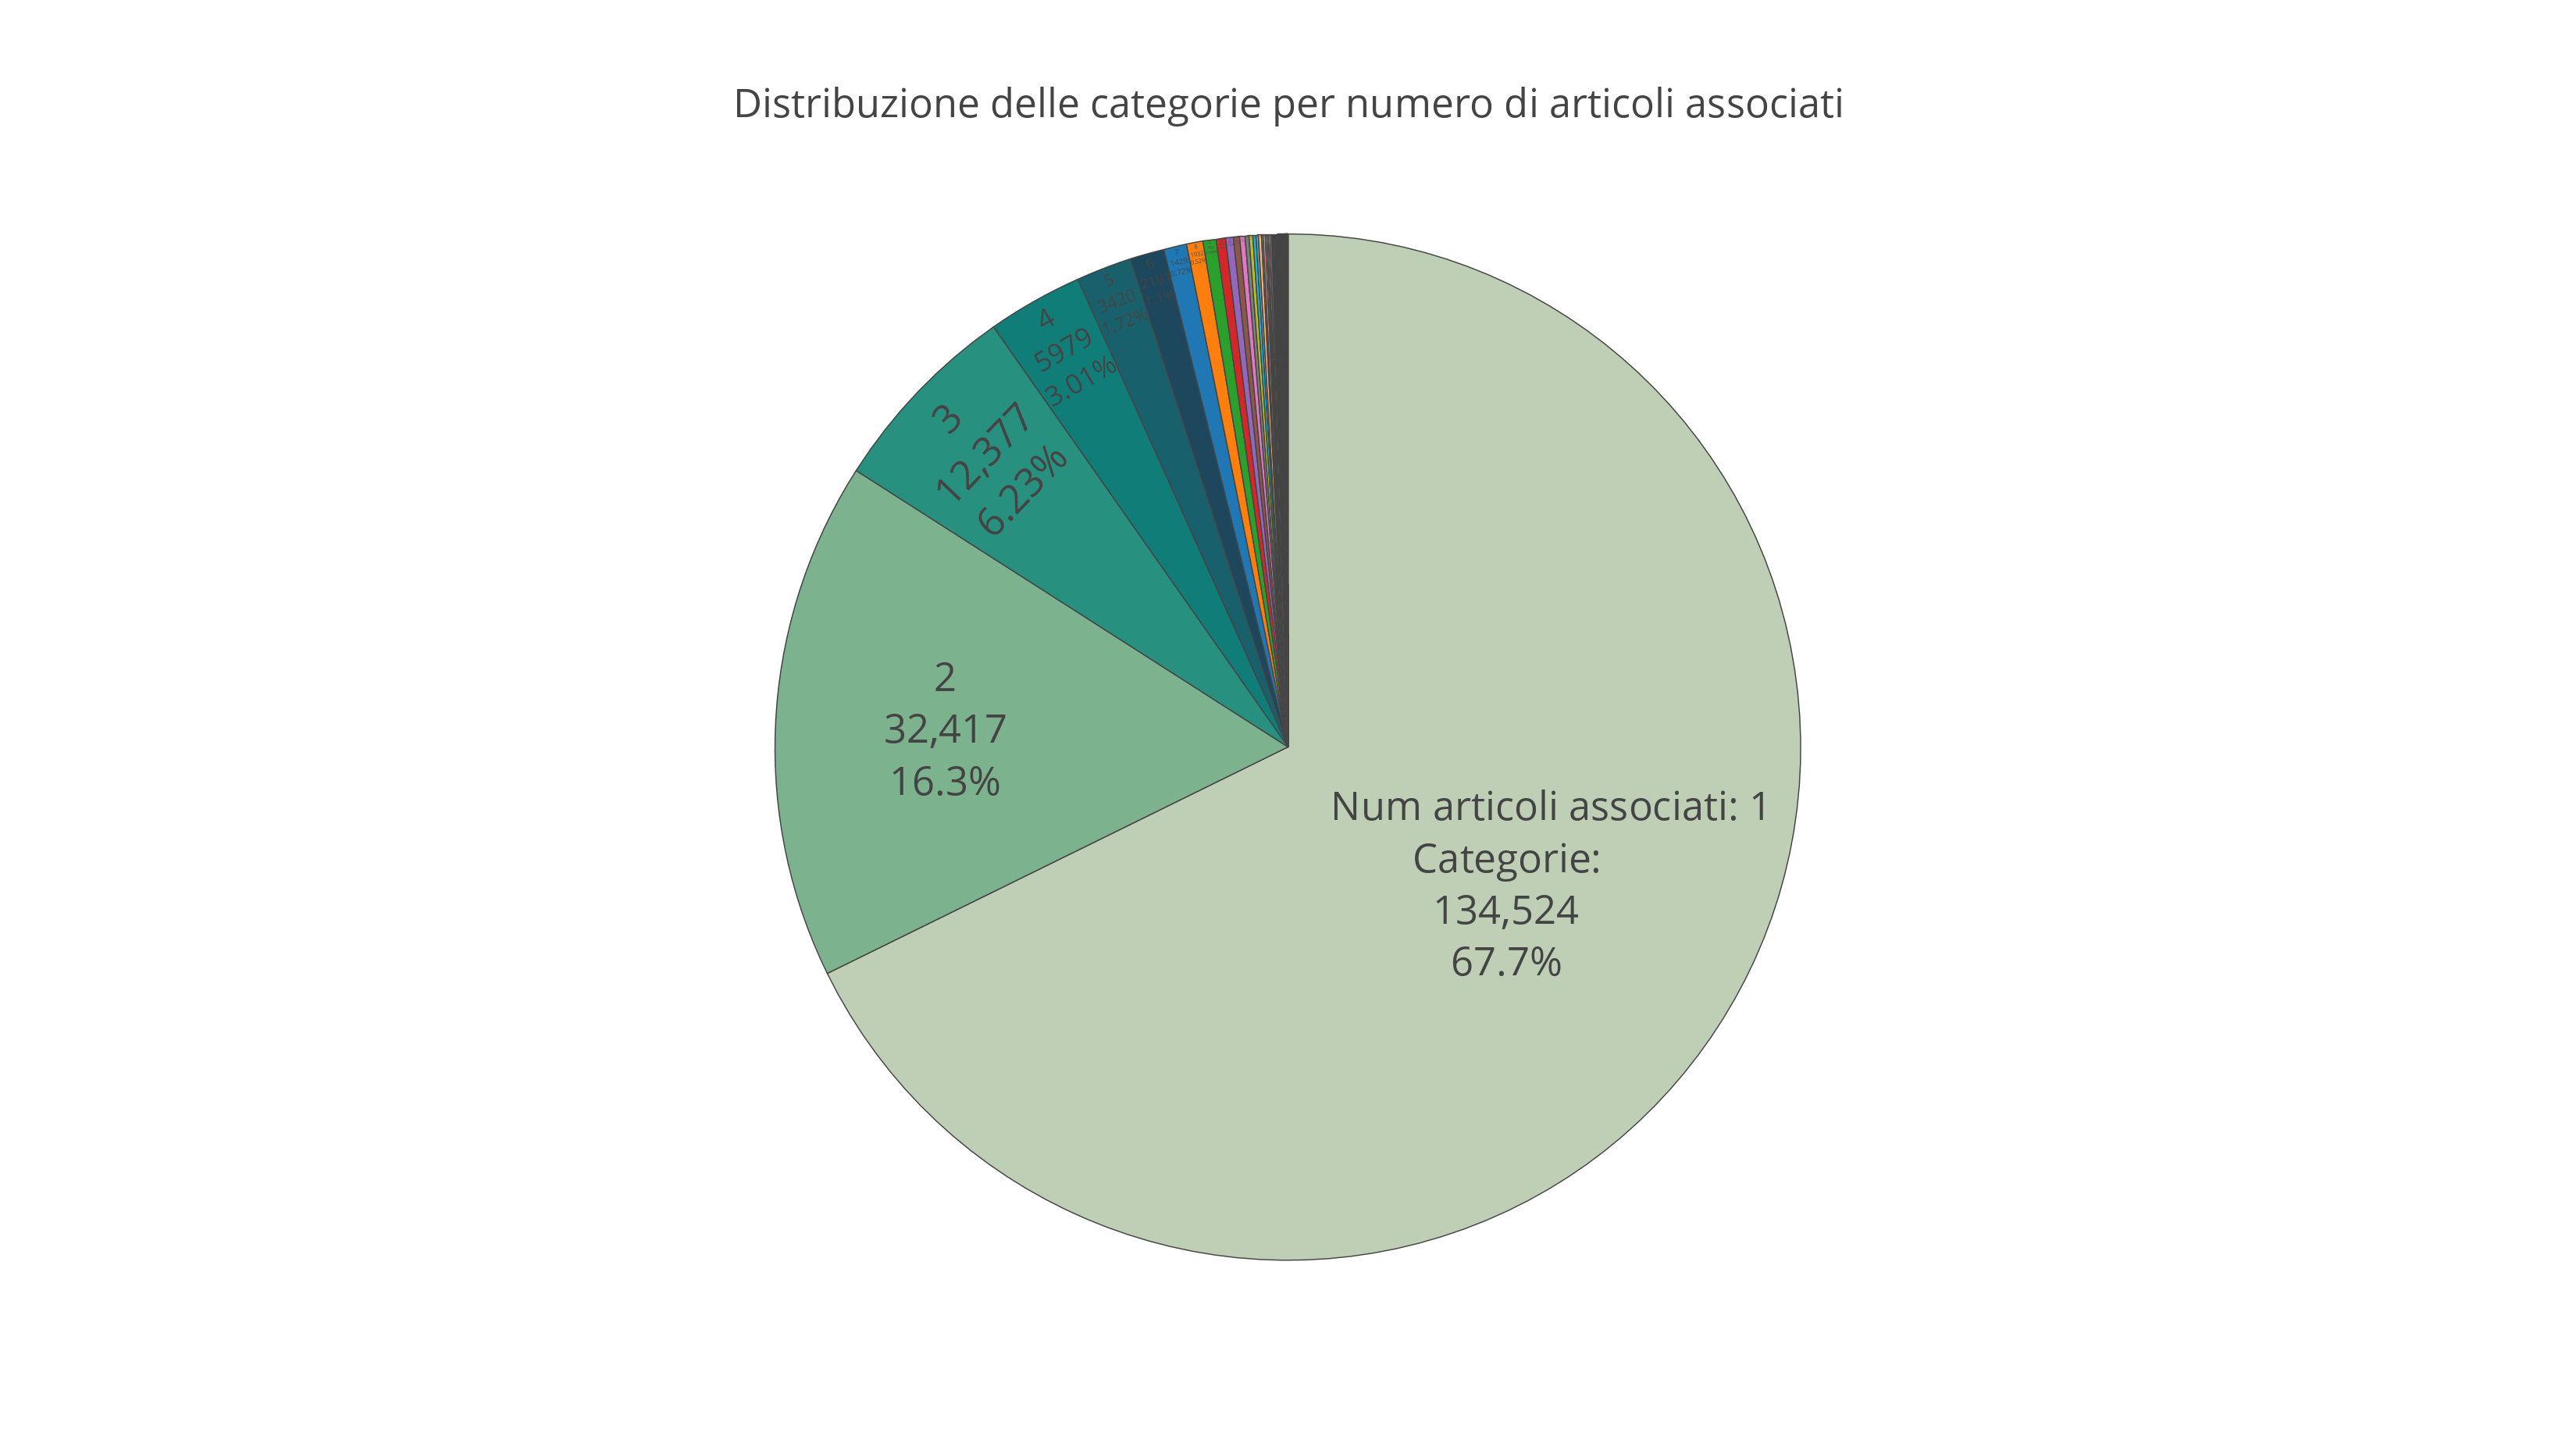
\includegraphics[scale=.5]{Figures/categoriesCake.png}
			\end{subfigure}
		\hspace{0.5cm}
			\begin{subfigure}{.5\textwidth}
			\centering
			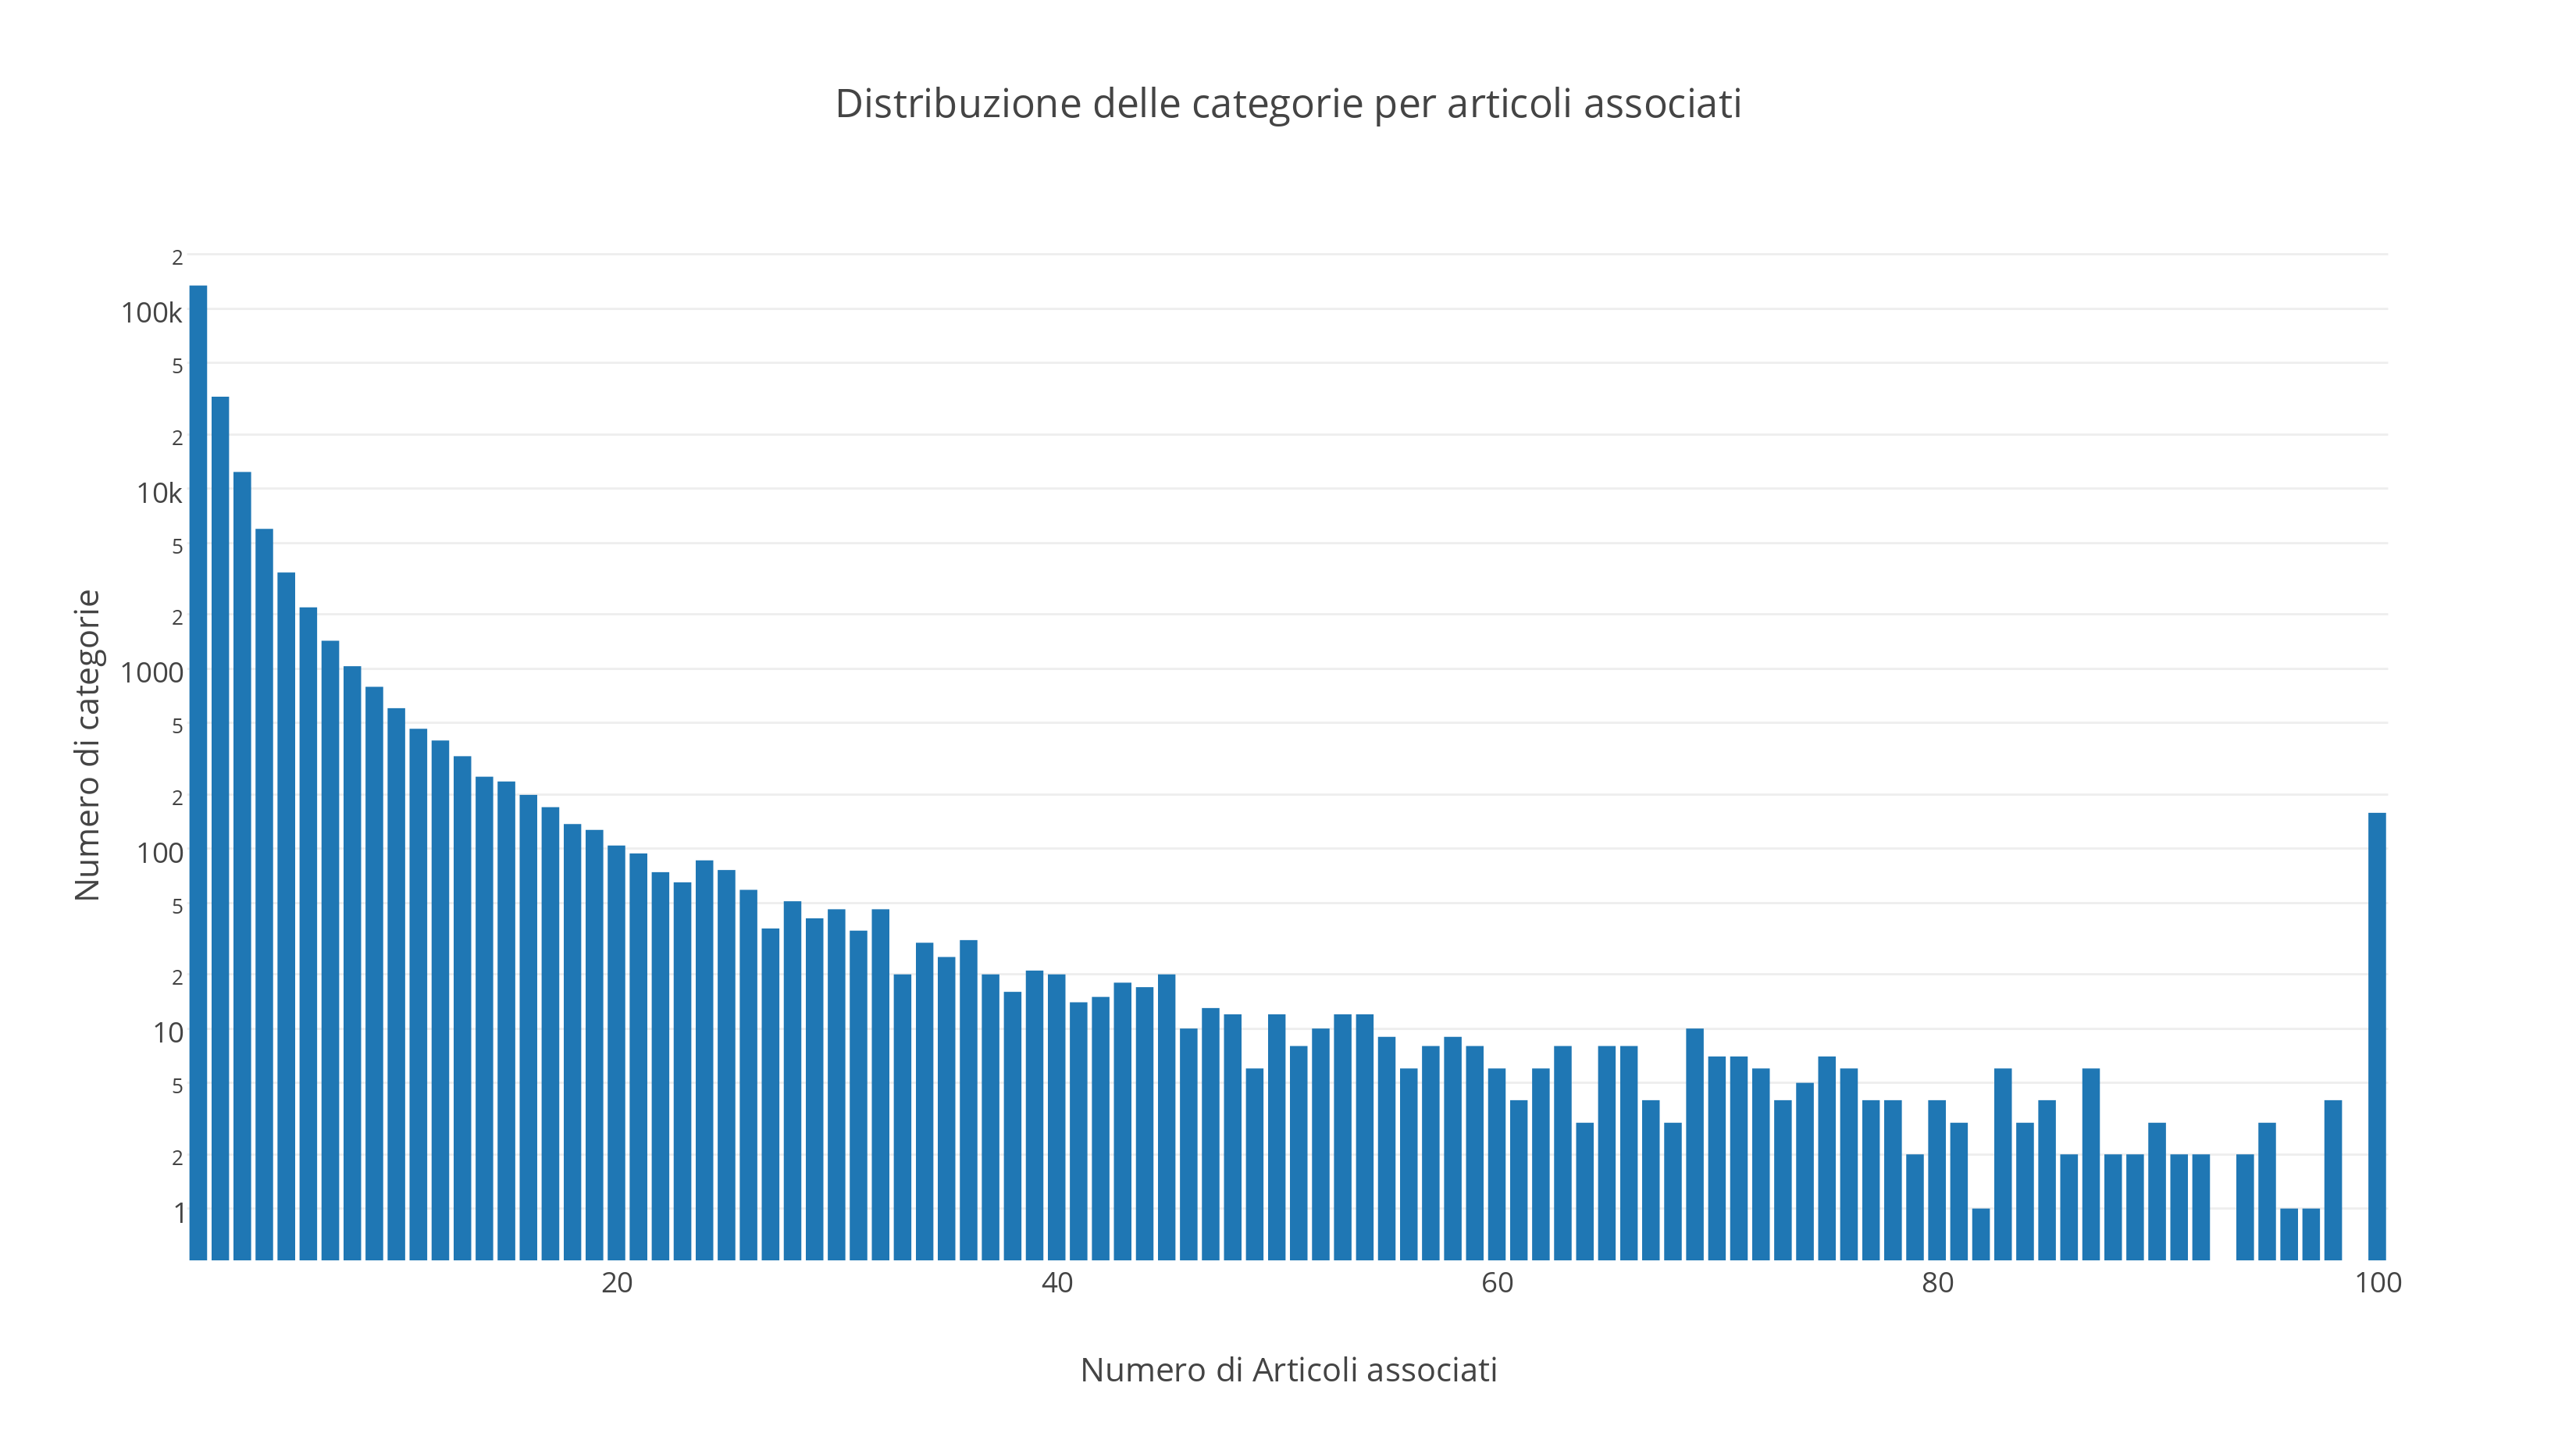
\includegraphics[scale=.5]{Figures/categories.png}
			\end{subfigure}
		\caption{Distribuzione delle categorie per numero di articoli. Nota: per rendere il grafico di destra leggibile il picco finale raggruppa il numero di categorie con cento o più articoli.}
		\label{fig:categories}
	\end{figure}

	L'analisi effettuata rivela infatti che, sul totale di 198.609 distinte categorie presenti nel dataset, circa due terzi (precisamente 134.524) di queste sono uniche, ovvero sono associate ad un solo articolo.
	Dato che queste non portano alcun contenuto informativo utile alla clusterizzazione, abbiamo provveduto ad escludere tali categorie dalle successive analisi.

	Nondimeno è anche presente un numero ristretto di 158 categorie associate a 100 o più articoli, le quali sono composte per lo più da categorie del genere "1900 deaths" e "1900 births" che si ripetono variando solamente l'anno.
	In tabella \ref{table:toptencategories} sono riportate a titolo di esempio le categorie con più articoli associati.


	\begin{table}[]
	%\hspace*{-2cm}
	\begin{tabular}{l|l||l|l}
	Living people & 14994 & Association football midfielders & 611 \\
	Year of birth missing (living people) & 1172 & Association football defenders & 502 \\
	Place of birth missing (living people) & 751 & Association football forwards & 409 \\
	American films & 741 & Year of birth unknown & 404 \\
	English-language films & 691 & English Football League players & 398 \\
	\end{tabular}
	\caption{Le categorie con maggior numero di articoli associati}
	\label{table:toptencategories}
	\end{table}


\section{Rappresentazione del Dataset}
	Prima di procedere con qualsiasi operazione sull'intero corpus si è deciso di preprocessare il data set eliminando le cosiddette \emph{stop words} presenti nel testo e lemmatizzando le parole rimaste.

	Per l'eliminazione delle \emph{stop words} ci siamo basati su una lista di parole fornita dal sito \url{http://www.ranks.nl/stopwords}.
	Questi termini vengono filtrati dal corpus in quanto portano un contenuto informativo sull'argomento dell'articolo pressochè nullo.

	La lemmatizzazione invece è stata eseguita utilizzando il $Lemmatizer$ di Spark al fine di raggruppare assieme le variazioni semantiche delle parole.

	\subsection{Vettorializzazione degli articoli}
		Per interagire con i più comuni algoritmi di clustering, ad esempio K-means, si è reso necessario trasformare gli articoli di Wikipedia in vettori.
		Per fare ciò abbiamo adottato una tecnica nota in letteratura con il nome \emph{Word2Vec}. Tale strumento, ideato da Tomas Mikolov, non è altro che una rete neurale a due strati il cui scopo è quello di trasformare parole del linguaggio naturale in vettori. Nello spazio vettoriale generato, le parole semanticamente più simili saranno più vicine, mentre parole che esprimono concetti differenti risulteranno distanti.

		Tale funzionalità è già implementata nella suite software di Spark, ma per sfruttarla al meglio è necessario settare alcuni parametri. Tra questi uno dei più importanti è la dimensione del vettore in uscita.
		In letteratura si è valutato che una dimensionalità nel ordine dei 100/300\cite{w2vdim} risulta un buon compromesso tra prestazioni e capacità di descrivere il dataset.

		Dopo aver allenato il modello \emph{Word2Vec} sul nostro corpus di testi, trasformando così le singole parole in vettori, ad ogni articolo è stata associata la media vettoriale di tutte le parole presenti nel suo testo. Il \emph{Basic Linear Algebra Subprograms} di Spark ci ha permesso di eseguire questa operazione molto rapidamente.

	\subsection{Bag of words} \label{sec:bag_of_words}

	L'algoritmo Bag of Words\cite{bagofwords} effettua la conversione degli articoli in vettori considerando le occorrenze dei termini in essi.
	In particolare viene considerata come metrica la \textit{Term frequency-inverse document frequency} (Tf-Idf).

	Si definisce la Tf-Idf relativa all'$i$-esimo termine nel $j$-esimo articolo come:
	$$ w_{i,j}=tf_{i,j}\times\log \left(\frac{N}{df_{i}} \right) $$
	dove $tf_{i,j}$ rappresenta il numero di occorrenze di $i$ in $j$, $df_{i}$ è il numero di documenti contenenti il termine $i$, ed $N$ è il numero totale di documenti.

	Abbiamo scelto di limitare l'analisi alle 3000 parole pi\`{u} frequenti nel dataset (escludendo le stopwords).

	Pertanto il modello prodotto associa ad ogni documento un vettore di dimensione 3000, contenente gli indici TfIdf associati ad ogni articolo per tutte le parole selezionate.

\section{Clustering}

	\subsection{Tecniche di Clustering}

		\subsubsection{Hopkins Statistic}
			Dopo aver effettuato la vettorializzazione dei documenti, si è cercato di stimare l'effettiva tendenza al clustering dei dati in nostro possesso utilizzando la statistica di Hopkins\cite{hopkins}.
			
			\vspace{5mm}
			\hfill\begin{minipage}{\dimexpr\textwidth-1cm}
			\begin{hopkins}
				Sia $X$ l'insieme degli $n$ punti del dataset, e se ne consideri un sottoinsieme random $\{x_1,...,x_m\}$ con $m \ll n$.
				Sia poi $Y$ un insieme generato di $m$ punti uniformemente distribuiti.
				Si definiscono quindi le distanze:
				\begin{itemize}
					\item $u_i$, distanza di $y_i \in Y$ dal pi\`{u} vicino punto di $X$
					\item $w_i$, distanza di $x_i \in X$ dal pi\`{u} vicino punto di $X$
				\end{itemize}
				La statistica di Hopkins \`{e} allora:
				
				$$H=\frac{\sum_{i=1}^m{u_i^d}}{\sum_{i=1}^m{u_i^d}+\sum_{i=1}^m{w_i^d}}$$
			\end{hopkins}
			\xdef\tpd{\the\prevdepth}
			\end{minipage}
			\vspace{5mm}
			
			Il dataset randomizzato necessario per la comparazione è stato generato basandosi sul dominio delle componenti dei vettori restituiti dalla vettorializzazione degli articoli mediante algoritmo \emph{Word2Vec}.

			Sono state eseguite svariate misurazioni di tale metrica utilizzando come sample una frazione da $0.1$ a $0.4$ dell'intero dataset e la statistica di Hopkins rilevata è stata compresa tra $0.011$ e $0.012$, valori che testimoniano una forte tendenza al clustering dei dati in nostro possesso.

		\subsubsection{K-means}
			Dato un insieme di punti $P \subset M$, dove $M$ è uno spazio metrico indotto da una funzione distanza $d$, l'algoritmo K-means punta a costruire una partizione $C = \{ C_1, ..., C_K \}$ con centri dei cluster $\{ c_1, ..., c_K\}$ che minimizzi la seguente funzione obiettivo.

			\begin{equation}
				\Phi_{K-means} (C) = \sum_{i=1}^K \sum_{p \in C_i \cap P} d(p, c_i) \\
			\end{equation}

			Per il nostro progetto abbiamo utilizzato l'implementazione Java \emph{KMeans} di Spark \emph{mllib}.

		\subsubsection{Latent Dirichlet Allocation}

			Latent Dirichlet Allocation (LDA)\cite{lda} è un modello generativo statistico che considera ogni documento come il risultato della sovrapposizione di più topic, individuati da un insieme di parole.

			Analogamente a k-means può essere utilizzata come algoritmo di clustering unsupervised associando gli articoli al topic avente influenza più alta nel loro corpus: questo permette non solo di individuare gruppi di articoli, ma di associare ad essi un contesto semantico.

			%TODO: Inserire tabella con un po' di topic significativi

			Nel nostro lavoro abbiamo scelto di usare 100 iterazioni per l'algoritmo in quanto oltre tale numero i miglioramenti nella qualità del clustering non sono rilevanti\cite{ldaiterations}, mentre come funzione obiettivo abbiamo scelto la log-likelihood\cite{ldaevaluation}.

			La complessità computazionale di questo metodo ci ha però limitati ad effettuare gli esperimenti con un numero di topic ridotto ($k=50,\,70,\,80$), avvicindandoci però a quanto suggerito da da \emph{K-means}.
			%TODO: valutare se metere anche altri k

		\subsubsection{Altri metodi}
			La libreria \emph{mllib} contiene altre tecniche, tra cui \emph{Gaussian mixture} e \emph{Bisecting k-means}, ma esse si sono rivelate inapplicabili, la prima per l'eccessivo tempo di calcolo e la seconda perché affine al già citato \emph{K-means}, ottimizzando infatti la stessa funzione obiettivo.


	\subsection{Valutazioni del Clustering}

		\subsubsection{Simplified Silhouette}
			\emph{Silhouette} è un metodo unsupervised per interpretare e validare un dato cluster.
			In particolare questa tecnica calcola per ogni punto la distanza media dal proprio cluster e la minima distanza media dagli altri cluster, valutando così sia la coesione che la separazione dei cluster, e restituisce un valore compreso tra $-1$ e $1$.

			Tale approccio però richiede tempo $\mathcal{O}(n^2)$, dove $n$ è la taglia dell'input, e il calcolo diretto risulta impraticabile a causa della taglia del dataset e le risorse di calcolo a nostra disposizione.

			Pertanto abbiamo provveduto a implementare e applicare una versione modificata che approssima questo l'algoritmo, denominata \emph{Simplified Silhouette}\cite{sscmapreduce}.

			Indicando con $a$ la distanza tra il punto considerato e il centro del proprio cluster e con $b$ la minima distanza tra il punto e gli altri centri del cluster, il {Simplified Silhouette Coefficient} è così definito:

			\begin{equation} \begin{aligned} \label{eq:simplifiedSilhouette}
				SSC = \frac{b - a}{ max(a, b) } = \frac{b - a}{b}
			\end{aligned} \end{equation}

			Si nota che il denominatore viene semplificato nel secondo passaggio.
			Ciò è possibile perché, per definizione dell'algoritmo \emph{K-means}, la distanza euclidea tra il punto e il suo centro sarà sempre minore della distanza tra il punto e un qualsiasi altro centroide.

			%Se così non fosse significherebbe che la distanza tra il punto considerato e il centroide di un altro cluster è minore che tra il punto e il centro del proprio cluster, ma questo è assurdo in quanto Kmeans forma i cluster proprio assegnando ogni punto al centroide più vicino.

			Questa approssimazione permette quindi di ottenere una buona stima di \emph{Silhouette}\cite{ssc} riducendo la complessità dell'algoritmo a $\mathcal{O}(Kn)$, dove $K$ è il numero di cluster e $n$ il numero di punti in input.

			Tale fattore di miglioramento delle prestazioni si indebolisce però all'aumentare di $K$, ritornando per $K \to n$ a una complessità quadratica.
			Nel caso generale tuttavia si cerca un numero di cluster minore di $n$ e \emph{Simplified Silhouette} porta ad un apprezzabile miglioramento di performance.

			Considerando la media dei coefficienti $SSC$ sui vari punti del dataset si ottiene infine un'indicazione globale sulla bontà del clustering.

			\smallbreak
			Un'ulteriore osservazione è il fatto che, con l'aumentare di $K$, il punteggio calcolato sia con \emph{Silhouette} che con \emph{Simplified Silhouette} tende a $1$ (il miglior punteggio possibile) e raggiunge effettivamente tale valore con $K = n$.
			In questo caso estremo ogni punto costituisce un cluster a sè stante e perciò $a$ si annulla portando a 1 il valore di $SSC$.

			Indicando con $d$ la distanza media tra il punto e il suo cluster e con $min(d)$ la minima distanza media tra il punto e gli altri cluster, si ha infatti che

			\begin{equation} \label{eq:silhouetteToOne}
				Silhouette = \frac{min(d) - d}{ max(d, \,min(d)) } \quad \xrightarrow [K \to n] \quad ~~ 1 \end{equation}

			Questo rende difficoltoso usare \emph{Silhouette} come strumento per individuare un $K$ ottimale, perché tende a provilegiare K elevati.
			Tale problematica può essere affrontata introducendo un peso al coefficiente restituito da Silhouette in maniera da evitare questa convergenza a $1$.
			Questa indagine esula tuttavia dagli scopi di questo lavoro non abbiamo trattato oltre questo punto che tuttavia può essere oggetto di studi futuri.

		\subsubsection{Normalized Mutual Information} \label{sec:NMI}
			L'informazione mutua è una quantità che misura la mutua dipendenza di due variabili aleatorie, ovvero quanta informazione porta sull'altra la conoscenza del valore di una delle due.
			Essa può essere impiegata per valutare quanto due partizioni, o \emph{clustering}, concordano nel suddividere un set di punti \cite{Manning}.

			Per fare questo, ad ogni cluster è stata associata una variabile indicatrice $\omega$, che assume valore 1 se il punto considerato appartiene al cluster e 0 altrimenti.
			Ogni clustering viene perciò individuato dall'insieme $\Omega$ di queste variabili aleatorie mutualmente esclusive e a somma unitaria.

			Con questa descrizione del problema è possibile calcolare l'informazione mutua tra due distinti clustering $\Omega$ e $\Phi$.
			Questa matrica è stata normalizzata in $(0, 1)$ per garantire un confronto alla pari tra clustering di dimensione diversa.
			NMI viene quindi definita come

			\begin{equation} \label{eq:NMI}
				NMI(\Omega, \Phi) = \frac
					{I(\Omega, \Phi)}
					{\left[ H(\Omega) + H(\Phi)\right] / 2}
			\end{equation}
			dove
			$$ I(\Omega, \Phi) =
					\sum_{\omega \in \Omega} \sum_{\phi \in \Phi}
						P(\omega \cap \phi) \log \frac {P(\omega \cap \phi)} {P(\omega) P(\phi)} $$
			$$ H(\Omega) = - \sum_{\omega \in \Omega} P(\omega) \log P(\omega), ~~~ H(\Phi) = - \sum_{\phi \in \Phi} P(\phi) \log P(\phi) $$

			All'atto pratico, come valore delle probabilità sono stati impegate stime a massima verosimiglianza, per esempio
			\begin{equation*}
				P(\omega) = \frac
					{ \text{numero di punti in }\omega }
					{ \text{numero di punti totali} }
			\end{equation*}.

			\smallbreak

			Purtroppo questa definizione non è direttamente applicabile al confronto tra cluster e categorie perché, mentre i clustering ottenuti con K-means e LDA sono delle effettive partizioni del dataset, non si può dire lo stesso delle categorie, dato che un articolo può possederne più di una.
			\smallbreak
			Il primo approccio per scogliere questo nodo è stato quello di eseguire un \emph{ranking} con \emph{Inverse Document Frequency} (vedi sezione \ref{sec:bag_of_words}) tra le categorie di ciascun articolo per eleggere la più rappresentativa.
			Grazie a questo passaggio NMI può essere calcolata direttamente dalla sua definizione (equazione \ref{eq:NMI}).
			\smallbreak
			Il secondo approccio tenta invece di estendere NMI al caso di cluster che si sovrappongano l'uno all'altro, considerando quindi ogni classe $c$ con la sua complementare $\bar{c}$ una partizione dell'insieme dei punti.

			L'informazione mutua viene calcolata quindi per ogni clustering $C = \{c, \bar{c}\}$ e si valuta la loro somma.

			\smallbreak
			I risultati sono presentati nella sezione seguente.

\section{Risultati}

	\subsection{Numero di cluster}
		Il clustering K-means risulta il più semplice e rapido da ottenere e per questo motivo abbiamo deciso di ispezionare un ampio range di valori per K, numero di cluster.

		La funzione obiettivo cala continuamente al variare del numero di cluster, come da figura \ref{fig:KMeansObj}, ma il calo diventa sempre più trascurabile al crescere di K.
		Questa osservazione è confermata dall'andamento della derivata della funzione obiettivo: essa raggiunge un tasso di incremento sostanzialmente nullo in prossimità del valore K=100.

		\begin{figure}[!htb]
			\hspace{-1cm}
			\begin{subfigure}{.5\textwidth}
				\centering
				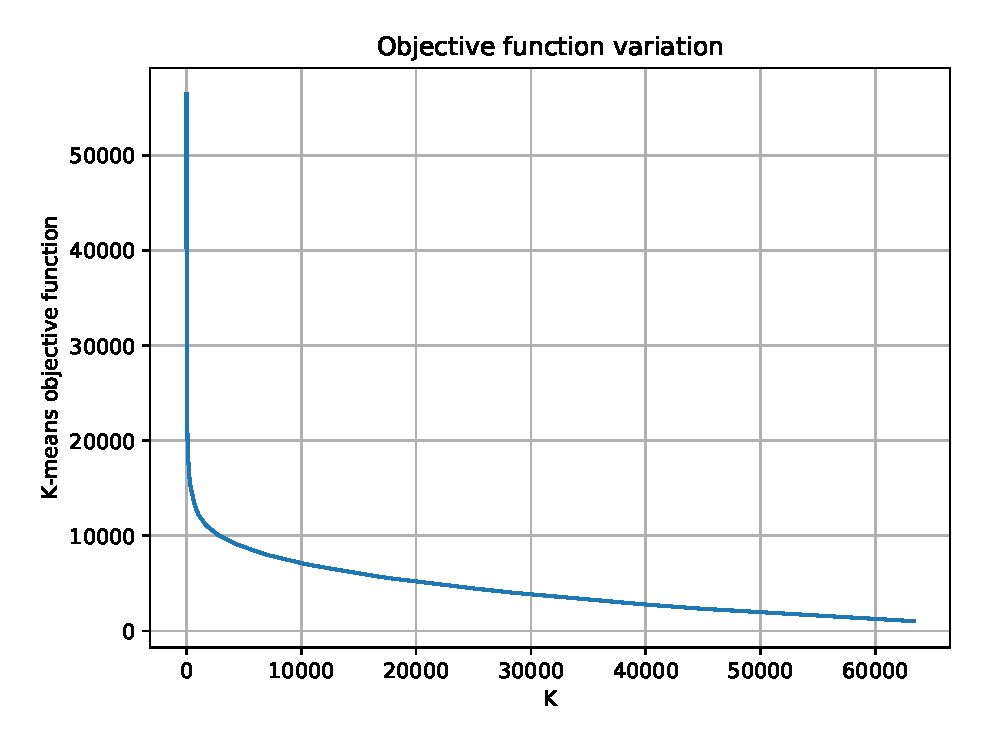
\includegraphics[scale=.5]{Figures/KMeans.eps}
			\end{subfigure}
			\hspace{0.5cm}
			\begin{subfigure}{.5\textwidth}
				\centering
				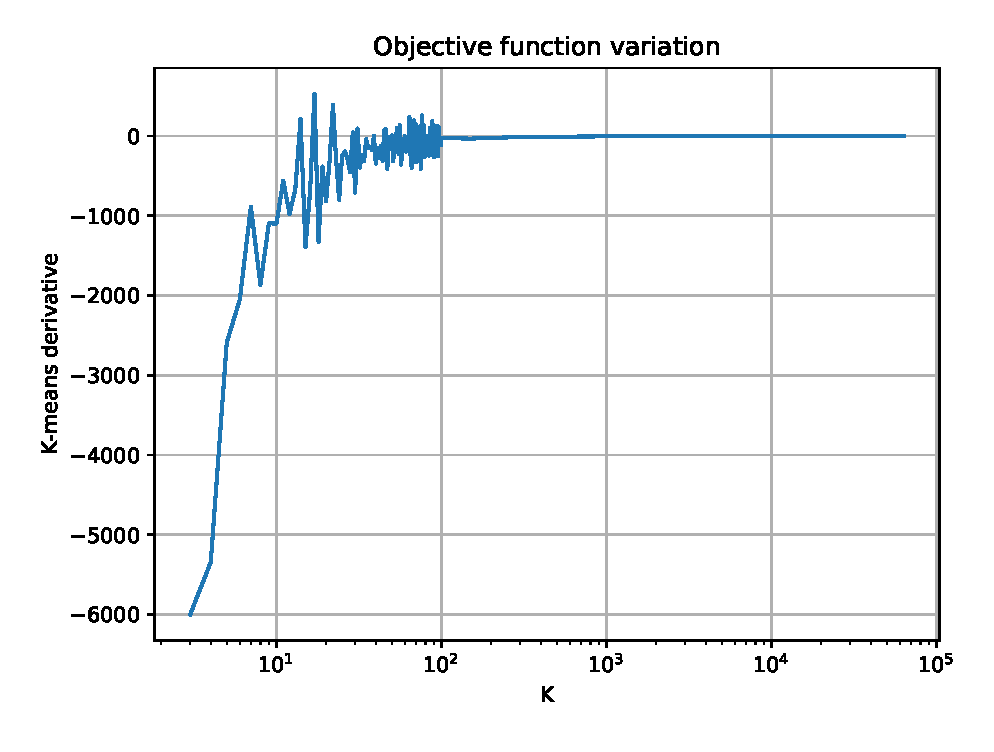
\includegraphics[scale=.5]{Figures/KMeansDerivative.eps}
			\end{subfigure}
			\caption{La funzione obiettivo smette di calare in modo significativo tra 50 e 150.}
			\label{fig:KMeansObj}
		\end{figure}

	Per questo motivo nelle analisi successive ci siamo concentrati su valori di K compresi tra 50 e 150.

	\subsection{Confronto tra i Cluster ottenuti con Normalize Mutual Information}
		Come si puo notare in figura \ref{fig:NMI-kmeans-categories}, l'andamento dell'informazione mutua del clustering rispetto alle categorie risulta analogo per entrambi gli approcci impiegati, descritti nella sezione \ref{sec:NMI}.

		L'aumento di informazione al crescere di K ci suggerisce che aumentando il numero di cluster il clustering si avvicina alla suddivisione indotta dalle categorie, ma che questo approssimarsi è tanto meno apprezzabile quanto più si sale con il valore di K.

		\begin{figure}[!htbp]
			\hspace{-1cm}
			\begin{subfigure}{.5\textwidth}
				\centering
				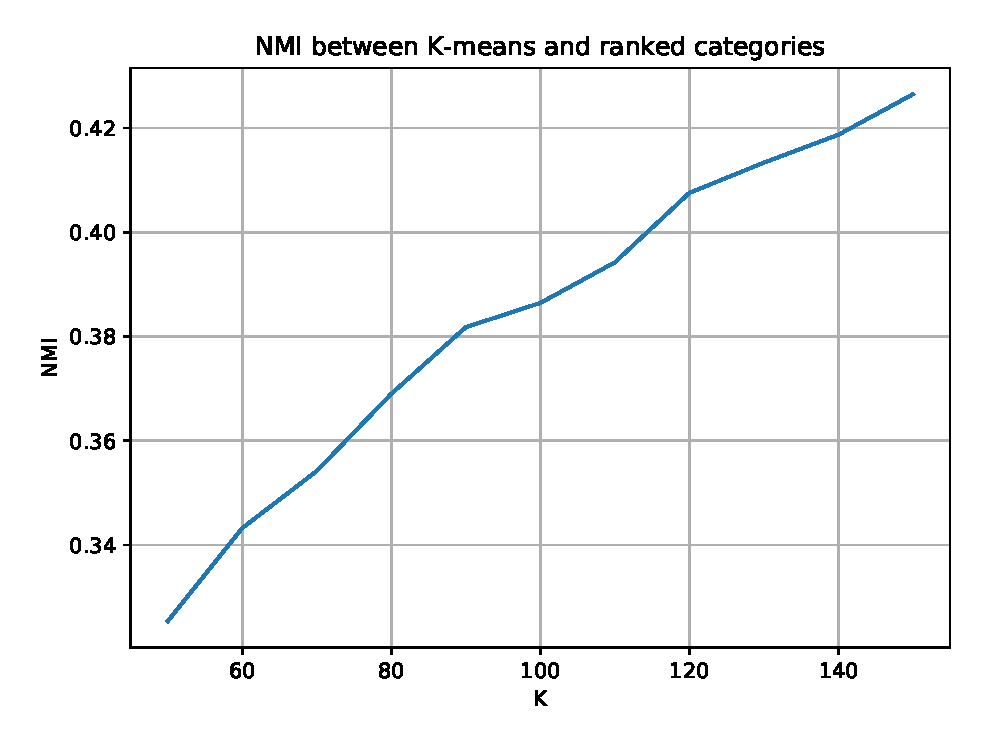
\includegraphics[scale=.5]{Figures/NMI-kmeans-ranked-categories.eps}
			\end{subfigure}
			\hspace{0.5cm}
			\begin{subfigure}{.5\textwidth}
				\centering
				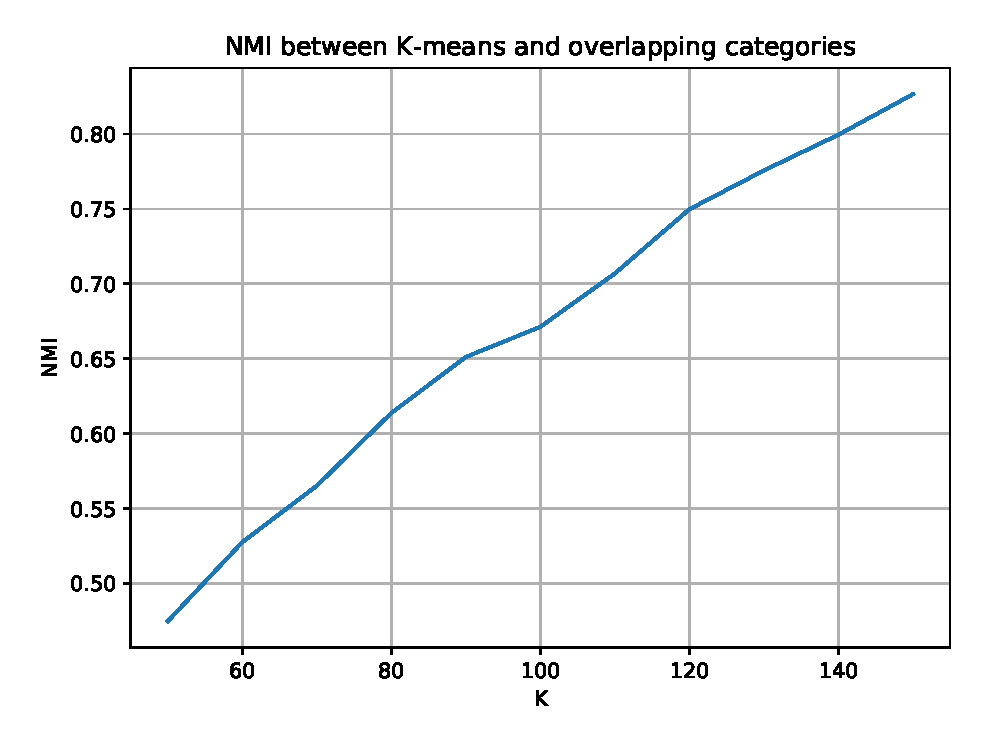
\includegraphics[scale=.5]{Figures/NMI-kmeans-overlapping-categories.eps}
			\end{subfigure}
			\caption{NMI tra K-means e il clustering indotto dalle categorie}
			\label{fig:NMI-kmeans-categories}
		\end{figure}

	\subsection{Validazione con Simplified Silhouette}
		Nel grafico \ref{fig:silhouetteValidation} sono riportati i valori per Simplified Silhouette, calcolati sui cluster generati da K-means al variare del numero di cluster.
		Si può notare come lo score, dopo un assestamento iniziale per cluster molto piccoli aumenti in maniera lineare arrivando ad uno score che si avvicina a $1$.
		Come riportato in precedenza tuttavia questo è dovuto più alla formulazione di Silhouette, che tende a $1$ per valore di $k$ vicino ad $n$, piuttosto che per un vero miglioramento del clustering.
        
		Si può comunque apprezzare una certa diminuzione della variazione della derivata per valori intorno a $k = 100$, pur rimanendo il fatto che in questo caso questa tecnica non porta da sola a risultati definitivi.
    
		\begin{figure}[!htb]
			\hspace{-1cm}
				\begin{subfigure}{.5\textwidth}
				\centering
				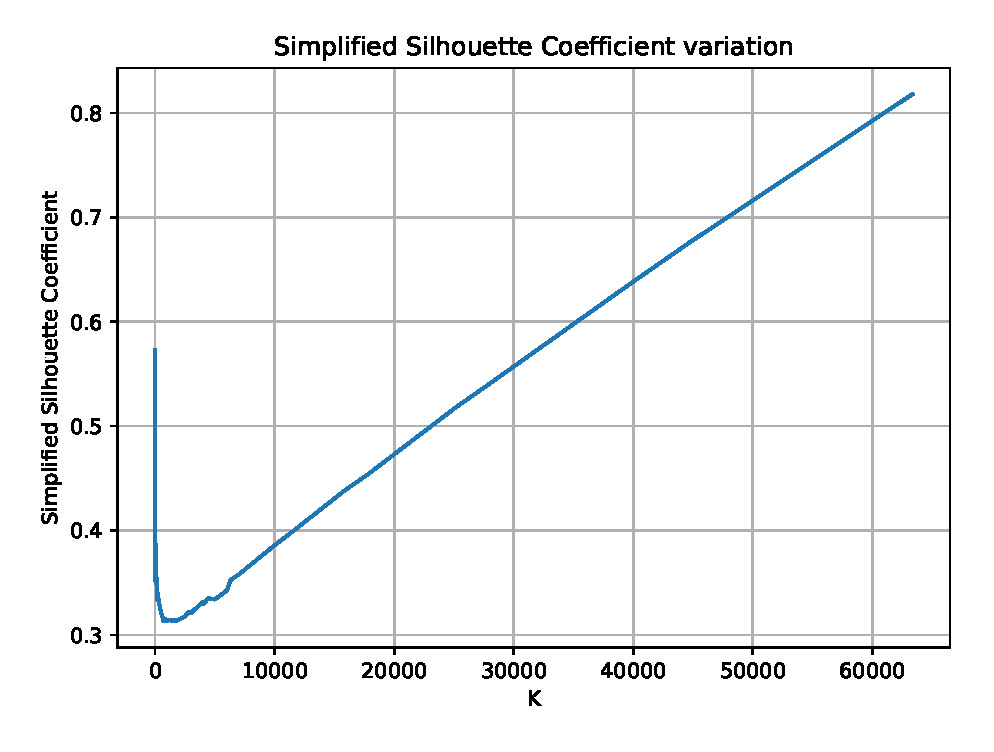
\includegraphics[scale=.5]{Figures/simplifiedSilhouette.eps}
				\end{subfigure}
			\hspace{0.5cm}
				\begin{subfigure}{.5\textwidth}
				\centering
				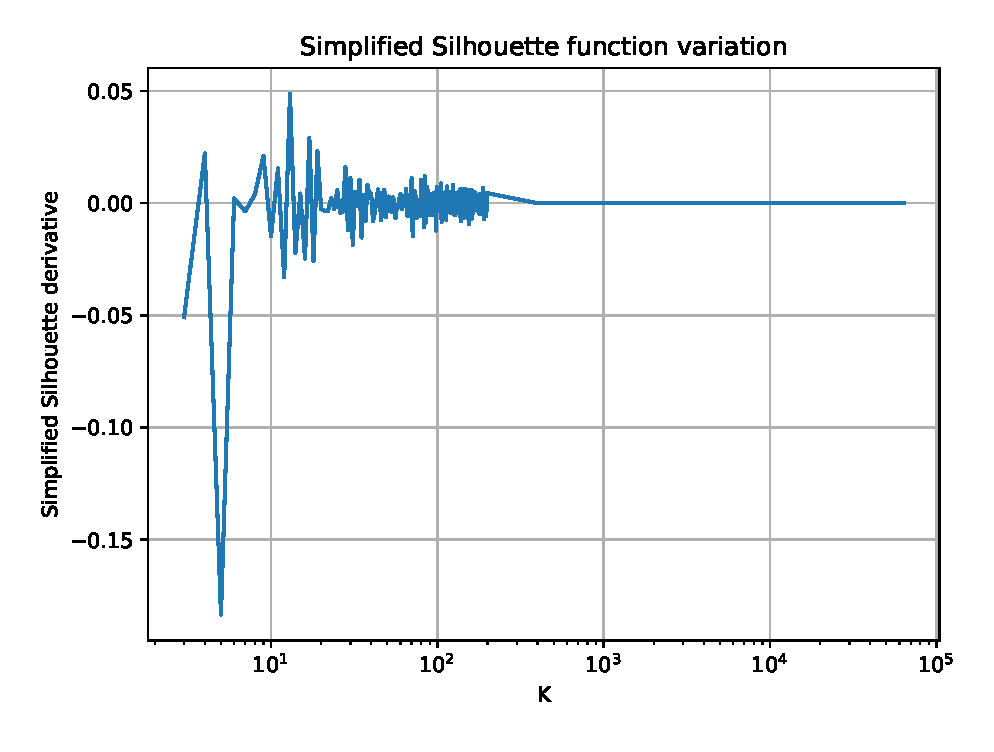
\includegraphics[scale=.5]{Figures/simplifiedSilhouetteDerivative.eps}
				\end{subfigure}
			\caption{Punteggio di Simplified Silhouette al variare di K e andamento della sua derivata.}
			\label{fig:silhouetteValidation}
		\end{figure}

\section{Conclusioni}
	Le conclusioni generali dalle analisi effettuate
	Proposte di punti da approfondire in studi futuri

%------------------------------------------------------------------------------
%	BIBLIOGRAPHY
%------------------------------------------------------------------------------

\begin{thebibliography}{12}

\bibitem{w2vdim}
    Tomas Mikolov, Kai Chen, Greg Corrado, and Jeffrey Dean. Efficient estimation of word representations
    in vector space. ICLR Workshop, 2013.

\bibitem{Manning}
	Christopher D. Manning, Prabhakar Raghavan and Hinrich Schütze, Introduction to Information Retrieval, Cambridge University Press. 2008

\bibitem{bagofwords}
	Harris, Zellig S. "Distributional structure." Word 10.2-3 (1954): 146-162.

\bibitem{hopkins}
	Banerjee, Amit, and Rajesh N. Dave. "Validating clusters using the Hopkins statistic." Fuzzy systems, 2004. Proceedings. 2004 IEEE international conference on. Vol. 1. IEEE, 2004.

\bibitem{lda}
	Blei, David M., Andrew Y. Ng, and Michael I. Jordan. "Latent dirichlet allocation." Journal of machine Learning research 3.Jan (2003): 993-1022.

\bibitem{ldainterpretation}
	Chang, Jonathan, et al. "Reading tea leaves: How humans interpret topic models." Nips. Vol. 31. 2009.

\bibitem{ldaevaluation}
	Griffiths, Thomas L., and Mark Steyvers. "Finding scientific topics." Proceedings of the National academy of Sciences 101.suppl 1 (2004): 5228-5235.

\bibitem{ldaiterations}
Wei, Xing, and W. Bruce Croft. "LDA-based document models for ad-hoc retrieval." Proceedings of the 29th annual international ACM SIGIR conference on Research and development in information retrieval. ACM, 2006.

\bibitem{sscmapreduce}
	Garcia, Kemilly Dearo, and Murilo Coelho Naldi. "Multiple parallel mapreduce k-means clustering with validation and selection." Intelligent Systems (BRACIS), 2014 Brazilian Conference on. IEEE, 2014.

\bibitem{ssc}
	Eler, Danilo Medeiros, et al. "Simplified Stress and Simplified Silhouette Coefficient to a Faster Quality Evaluation of Multidimensional Projection Techniques and Feature Spaces." Information Visualisation (iV), 2015 19th International Conference on. IEEE, 2015.

\end{thebibliography}

%----------------------------------------------------------------------------------------

\end{document}
